

\chapter{Multivariable Optimization Theory}

\section{Matrix Differentiation}

\begin{theorem}
    Given a constant matrix $\MA$:
    $$\frac{\partial}{\partial\vy}(\vy^\intercal\MA\vy) = \vy^\intercal(\MA + \MA^\intercal)$$
\end{theorem}
\begin{theorem}
    For functions $f$ and $g$ and matrix $\MA$ with compatible dimensions:
    $$\frac{\partial}{\partial\vy}f(\vy)^\intercal\MA g(\vy) = g(\vy)^\intercal\MA^\intercal\frac{\partial}{\partial\vy}f(\vy) + f(\vy)^\intercal\MA\frac{\partial}{\partial\vy}g(\vy)$$
\end{theorem}

\section{Optimization Theory} \label{optim}

\subsection{Optimization with No Constraints} 

\subsection{Constrained Optimization}

In the previous sections, we discussed optimization problems looking for solutions in $\mathbb{R}$ to attain the maximum or minimum value of a function. Sometimes, we want to optimize f over some restriction of its domain. For example, we may want to satisfy a financial budget for a project. These problems are called $\define{constrained optimization}$ problems.

\begin{definition}\label{def_constrained_optimization} 
A \define{constrained optimization} problem is an optimization problem for which we want to find the maximal or minimal value of a function $f(\vx)$ over a subset of all possible values of $\vx$. An optimization problem that is not constrained is called an \define{unconstrained optimization} problem.
\end{definition}

Consider $f:\mathbb{R}^n\rightarrow\mathbb{R}$ and a set $S \subseteq \mathbb{R}^n$. We want to find:
$$x^*=\underset{\vx \in S}{\argmin} f(\vx)$$
or 
$$f_{min} = \min_{\vx \in S} f(\vx)$$

One approach is to modify the gradient descent algorithm. At each step, we check if $f(\vx)$ is in $S$. If it is not, then we project $\vx$ back into $S$ before taking the next step. Unsurprisingly, this is called \define{projected gradient descent}. One way to do the projection is to find the value $\vx\in S$ such that:

$$ \underset{\vx \in S}{\argmin} \norm{\vx - \vx_{i-1}}$$
where $\vx_{i-1}$ is the result of the previous gradient descent step and is not in $S$. \\

Note that the projection step is another optimization problem. When our constraint is simple, projected gradient descent is a useful method. However, when our constraint set $S$ is complicated, determining the projection step may add significant overhead to our algorithm. Examples for which projected gradient fails will be explored in exercise JANICE (In solution, talk about convexity. If Q is a convex set, the optimization problem has a unique solution.
I If Q is nonconvex, the solution to PQ(x0) may not be unique: it gives
more than one solution.)!!!. In these cases, we'd hope to use a different constrained optimization method. 

One such approach is to construct an unconstrained optimization problem whose solutions are able to be transformed into solutions of the original, constrained problem. This can be done in many ways. We will discuss the \define{Karush-Kuhn-Tucker} (KKT) method, which constructs a new problem with identical solutions to the original.

In order to apply KKT, $S$ must be describable in the following way:
$$S = \{\vx | g_i(\vx)=0 \textrm{ and } h_j(\vx) \leq 0 \textrm{ for  }1\leq i \leq n \textrm{, } 1\leq j\leq k\}$$

Then, we may construct the following function:

\begin{definition}
Define the \define{Lagrangian} to be the function $L(\vx;\vlambda,\valpha)$ such that
$$L(\vx;\vlambda,\valpha) = f(\vx) + \sum_{i} \lambda_{i} g_{i}(\vx) + \sum_{i} \alpha_{i} h_{i}(\vx)$$
The parameters $\valpha$ and $\vlambda$ are called  \define{KKT multipliers}. The equalities involving $g_{i}$ are called the \define{equality constraints}, and the inequalities involving $h_{i}$ are called the \define{inequality constraints}.
\end{definition}

\begin{remark}
In the case where $S$ can be described exclusively by the equality constraints, the Lagrangian reduces to $$L(\vx;\vlambda) = f(\vx) + \sum_{i} \lambda_{i} g_{i}(\vx)$$ In this case, $\vlambda$ is called the \define{Lagrangian multiplier}. 
\end{remark}

\begin{proposition}
Let $S$, $L(\vx;\vlambda,\valpha)$ be defined as described in the KKT method. Then, 
$$\min_{\vx \in \mathbb{R}^n} \max_{\vlambda} \max_{\valpha : \valpha \geq 0} L(\vx;\vlambda,\valpha)$$
has the same solutions as $\min_{\vx\in S} f(\vx)$.
\end{proposition}

The justification is as follows:

If $\vx \notin S$, then $g_{i}\neq 0$. The parameter $\vlambda$ is unbounded by definition, resulting in 
$$\max_{\vlambda} \max_{\valpha : \valpha \geq 0} L(\vx;\vlambda,\valpha)=\infty$$
So, any $\vx \notin S$ cannot be an optimal solution.

If $\vx \in S$, then $\sum_{i}\lambda_{i} g_{i}(\vx) = 0$. Note that since $\valpha\geq0$ by definition, we also have $\max_{\valpha : \valpha \geq 0} \valpha_{i} h_{i}(\vx) = 0$. So,   
$$\max_{\vlambda} \max_{\valpha : \valpha \geq 0} L(\vx;\vlambda,\valpha) = f(\vx)$$ 
Thus when $\vx \notin S$, $\vx$ cannot be an optimal solution for $\min_{\vx\in S} f(\vx)$, and when $\vx \in S$, the optimal solutions are equivalent. 

\begin{remark}
We can construct the Lagrangian to adjust the maximums and minimums involved:

$$\min_{\vx} \max_{\vlambda} \max_{\valpha : \valpha \geq 0} -f(\vx) + \sum_{i} \vlambda_{i} g_{i}(\vx) + \sum_{i} \valpha_{i} h_{i}(\vx)$$

$$\max_{\vx} \min_{\vlambda} \min_{\valpha : \valpha \geq 0} f(\vx) + \sum_{i} \vlambda_{i} g_{i}(\vx) - \sum_{i} \valpha_{i} h_{i}(\vx)$$
\end{remark}

Now, we have reduced our constrained optimization problem to an unconstrained optimization problem. However, not all Lagrangian optimization problems can be easily solved. Fortunately, the KKT method also provides us with a set of conditions that describe the optimal solutions. 

\begin{theorem}[Karush-Kahn-Tucker Conditions]\label{Karush-Kahn-Tucker Conditions}\
Let $f:\mathbb{R}^n \to \mathbb{R}$ and $S\in\mathbb{R}^n$. Let $L(\vx;\vlambda,\valpha)$ be a Lagrangian function for $f$, $S$. If $\vx$ is a solution for $\underset{\vx\in\mathbb{R}^n}{\argmin} f(\vx)$, then the following are true:
    \begin{itemize}
        \item $\nabla{x} L(\vx;\vlambda,\valpha) = 0$
        \begin{itemize}
            \item In the case where $f$ is not differentiable, the gradient is defined as a set of possible slopes, and this conditions states that $0$ is an element of the gradient.
        \end{itemize}
        \item $\vx \in S$ and the constraints on the KKT multipliers are satisfied.
        \item $\sum_{i} \alpha_{i} h_{i}(\vx)=0$ (this is also known as the \define{complementary slackness} condition).
        \end{itemize}
\end{theorem}

These conditions sometimes allow us to determine the solution analytically. If we are unable to analytically determine the solution, these conditions still give us useful information for computing the solution numerically. 

\section{Convex Optimization} 


\subsection{Convex Functions}
\label{convex-functions}
\begin{definition}
    \label{def-convexity}
    A function $f : \R^n \rightarrow \R$ is \define{\cvx} if for all $\vx, \vy \in \R^n$ and all $0 \leq t \leq 1$ we have:
    $$f(t\vx + (1-t)\vy) \leq tf(\vx) + (1-t)f(\vy)$$
    and $f$ is strictly \cvx{} if
    $$f(t\vx + (1-t)\vy) < tf(\vx) + (1-t)f(\vy)$$
    Intuitively, $f$ is \define{\cvx} if the line segment between any two points on the graph function is above the graph between the two points.
\end{definition}

\begin{example}
    Example of the convexity of the function $f(x) = \frac{1}{2}x^2 -3x+5$
    \begin{center}
      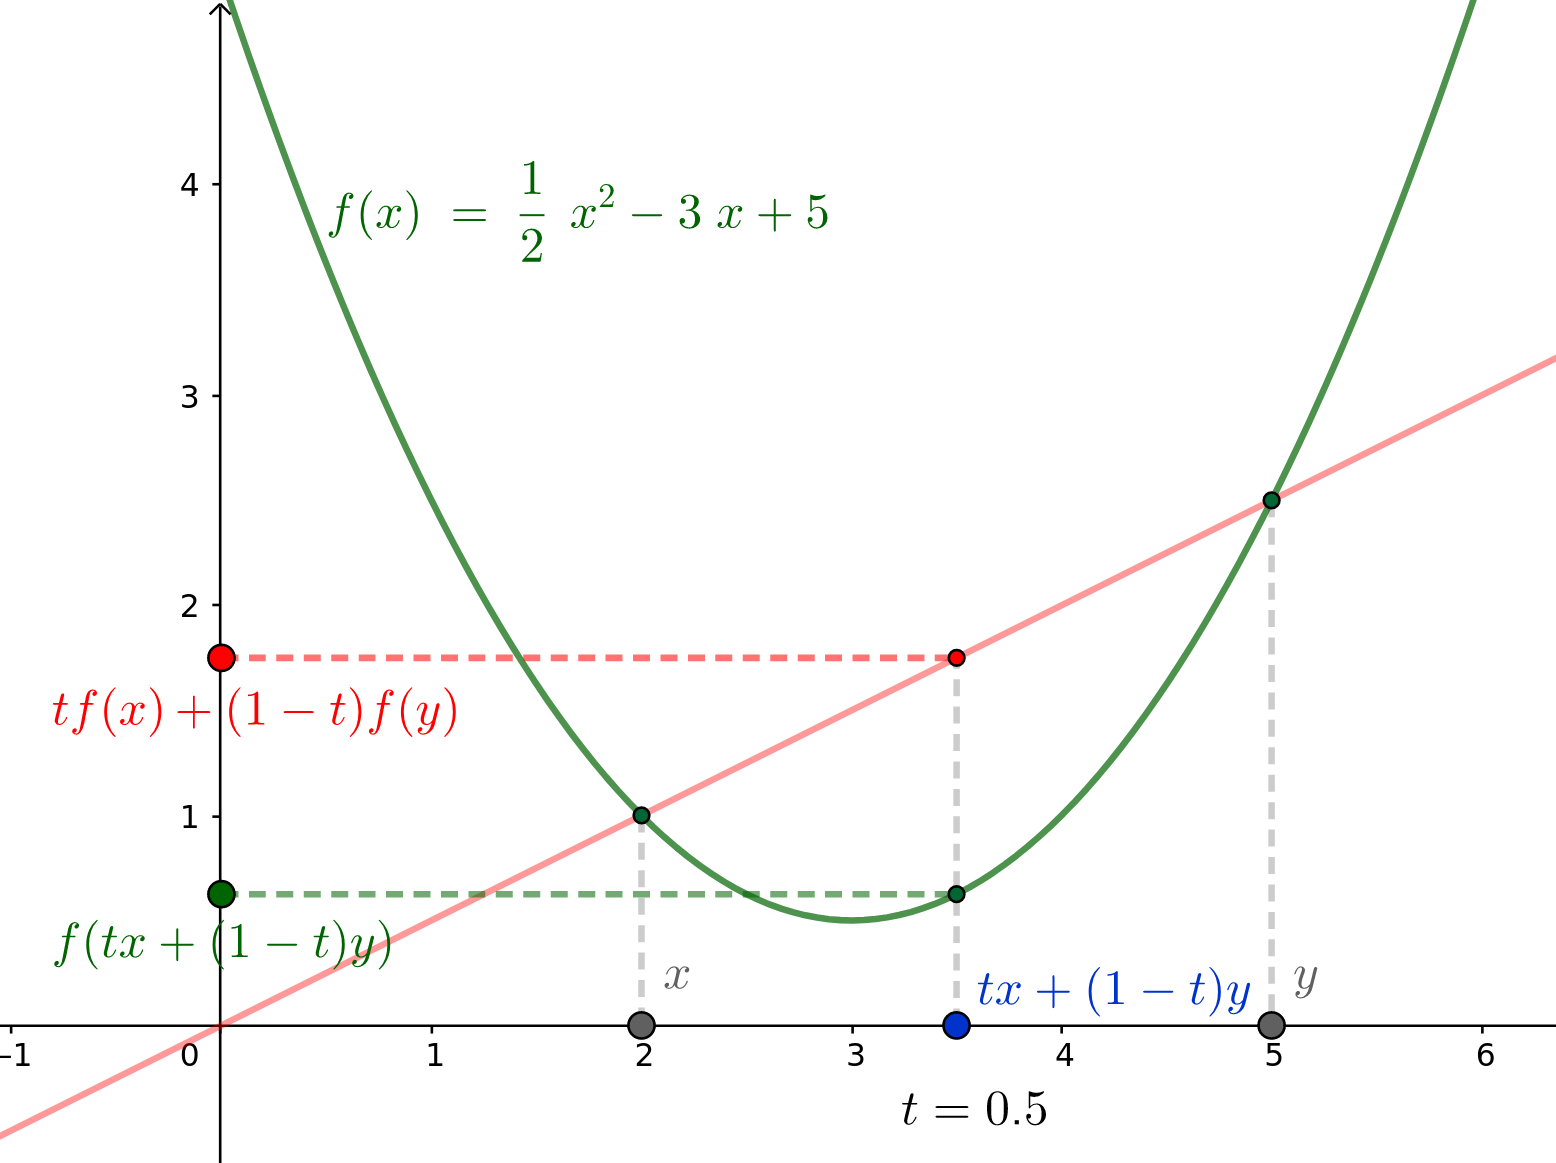
\includegraphics[width=4in]{images/Chapter4/convex1.png}
    \end{center}
    
    Here we clearly see that :
    \begin{itemize}
        \item $f(tx + (1-t)y) \leq tf(x) + (1-t)f(y)$
        \item The line segment between f(x) and f(y) is above the graph between these two points
    \end{itemize}
    
    To prove that $f$ is \cvx, this must be true for all $x$ and $y$.
\end{example}

This definition of convexity applies to functions that are not necessarily differentiable, which is sometimes the case with the functions used in deep learning. For example, an often used activation function is ReLu (Rectified Linear Unit), which is not differentiable.

\begin{example}
    Let's show that $f(x) = \abs{x}$, is \cvx. To do so, we can use the above definition of convexity. Let $x,y \in \R$ and $t \in [0,1]$:
    \begin{ceqn}
    \begin{align*}
    f(tx + (1-t)y) &= \abs{tx + (1-t)y} \\
    &\leq \abs{tx} + \abs{(1-t)y} \text{ \hspace{5mm} using the triangle inequality} \\
    &= t \abs{x} + (1-t)\abs{y} \text{\hspace{5mm} as $t \in [0,1]$} \\
    &= tf(x) + (1-t)f(y)
    \end{align*}
    \end{ceqn}
    We have $f(tx + (1-t)y) \leq tf(x) + (1-t)f(y) $ so $f$ is \cvx. 
\end{example}

\begin{proposition}
    \label{convex-property}
    A differentiable function $f: \R \to \R$ is \cvx{} if and only if its graph lies above all of its tangents:
    $$f(y) \geq f(x) + f'(x)(y-x), \forall x,y \in \R$$
    This property can be generalized to functions of several variables. For functions $f: \R^n \to \R$, this becomes
    $$f(\vy) \geq f(\vx) + \nabla_\vx f(\vx) \cdot (\vy - \vx)$$
\end{proposition}

\begin{remark}
    This property means that the first Taylor expansion at any point of a \cvx{} function, is a global under-estimator of the function.
\end{remark}

\begin{example}
    Example with the same function $f(x) = \frac{1}{2}x^2 -3x+5$
    \begin{center}
      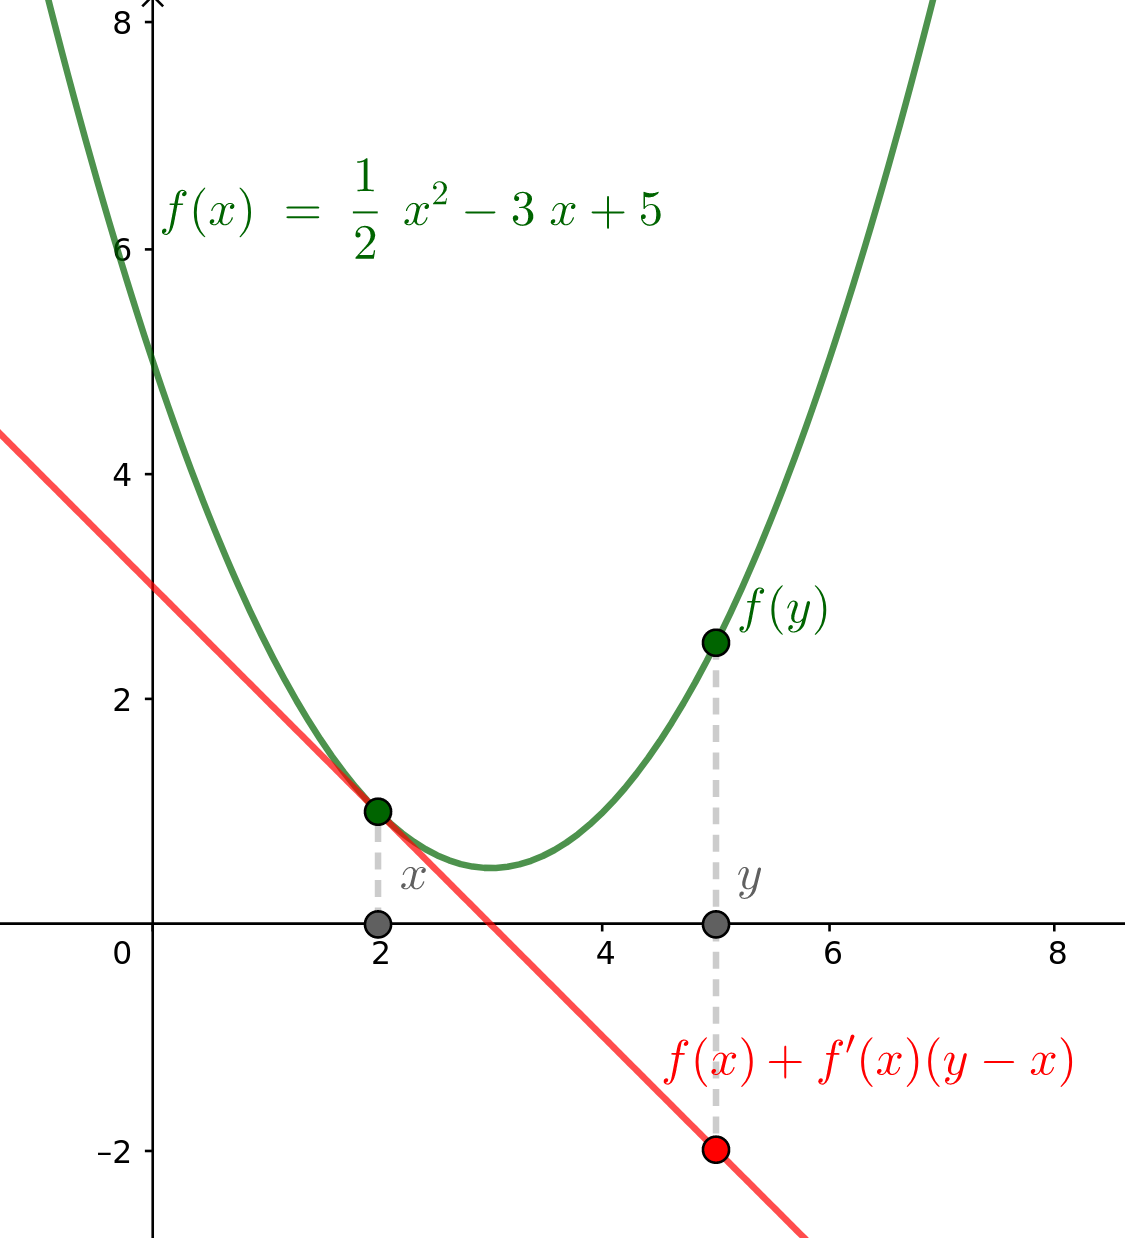
\includegraphics[width=3in]{images/Chapter4/convex2.png}
    \end{center}
    Here we clearly see that :
    \begin{itemize}
        \item $f(y) \geq f(x) + f'(x)(y-x)$
        \item The graph lies above the tangent on $x$.
    \end{itemize}
    Again, to prove that $f$ is \cvx, this must be true for all $x$ and $y$.
\end{example}

\begin{theorem}
    \label{theorem-hessian-convex}
    A twice differentiable function $f : \R^n \rightarrow \R$ is \cvx{} if and only if $H(f)(\vx)$ is positive semi-definite for all $\vx \in \R^n$. If $H(f)(\vx)$ is positive definite, then $f$ is strictly \cvx.
\end{theorem}

\begin{remark}
    One way to see this theorem, is that the first derivative of a  \cvx{} function is always increasing, so the second derivative is always positive.
\end{remark}


\subsection{Consequences of Convexity}


\begin{definition}
A function $f: \R^n\rightarrow\R$ is $\mathcal{L}$-Lipschitz continuous if $\exists \mathcal{L}>0$, such that $\forall \vec{x}, \vec{y}\in \R^n$,$||f(\vec{x})-f(\vec{y})||\geq \mathcal{L}||\vec{x}-\vec{y}||_2$
\end{definition}

\begin{example}
Suppose constant A $\in \R^n$ that is greater than 0.
\begin{align}
    f(\vec{x})&=A\vec{x}+\vec{b}\\
||f(\vec{x})-f(\vec{y})||&=||A\vec{x}+\vec{b}-A\vec{y}-\vec{b}||\\
&=||A(\vec{x}-\vec{y})+\vec{b}-\vec{b}||\\
&=A||(\vec{x}-\vec{y})||
\end{align}
Since A is a constant, there must exist an $\mathcal{L}$ that is less than or equal to $A$, implying 
\begin{equation}
    A||(\vec{x}-\vec{y})||\geq A||(\vec{x}-\vec{y})||
\end{equation}. Thus $f(\vec{x})$ must be $\mathcal{L}$-Lipschitz continuous.
\end{example}

\begin{definition}
$f: \R^n\rightarrow\R$ is convex if $H(f)(\vec{x}))$ is a positive semidefinite for all $\vec{x}\in \R$
\end{definition}

\begin{example}
Consider $f(\vec{x})=b^T\vec{x} +\vec{x}^T A\vec{x}+c$
\begin{align*}
\frac{df}{d\vec{x}}(\vec{x})&=b^T+\vec{x}(A+A^T)\\
&=b^T+2\vec{x}^TA\\
&=\frac{df}{d\vec{x}^2}(\vec{x})=2A^T=2A
\end{align*}
so f is convex iff A is positive semi-definite
\end{example}

\begin{example}
$f(\vec{x})=x^T\vec{x}={||\vec{x}||^2}_2$ is convex $\vec{x}$
\end{example}


\section{Exercises}



\begin{enumerate}
    \item Let $f(x) = \frac{1}{2} x^T A x + b^T x$ where $A$ is a symmetric matrix and  $b \in \mathbb R^n$ is a vector. What is $\nabla_x f(x)$? What is $\nabla^2_x f(X)?$
    \item Let $f(x) = g(h(x))$ where $g: \mathbb R \rightarrow R$ is differentiable and $h : \mathbb R^{n} \rightarrow \mathbb R$ is differentiable. What is $\nabla_x f(x)$? 
    \item Let $f(x) = g(a^T x)$ where $g : \mathbb R \rightarrow \mathbb R$ is continuously differentiable and $a \in \mathbb R^n$ is a vector. What is $\nabla_x f(x)$ and $\nabla^2 f(x)$?
    \item Consider the average empirical loss (the risk) for logistic regression: 

    $$J(\theta) = \frac{1}{m} \sum_{i = 1}^m \log(1 + e^{- y^{(i) \theta^T x^{(i)}} } = \frac{-1}{m} \sum_{i = 1}^m \log(h_{\theta}(y^{(i) x^{(i)}})$$
    where $h_{\theta}(x) = g(\theta^T x)$ and $g(z) = \frac{1}{(1 + e^{-z})}$. 
    \begin{enumerate}
    \item Find the Hessian $H$ of $J(\theta)$. 
    \item Should that $H$ is positive semi-definite. 
    \end{enumerate}
        \item To prove the theorem (\ref{proof-theoreme-gd-converge}), we use the proposition (\ref{convex-property}) about the tangents of \cvx{} functions. Prove this proposition by showing that $\forall x,y \in \R$ we have $$f(y) \geq f(x) + f'(x)(y-x) \equiv f \text{ is \cvx}$$
            \item Let $F: \R^3 \to \R$ defined by $F(x,y,z) = x^2 + y^2 + z^2 - xy -z$. Show that $F$ is \cvx{} using the theorem (\ref{theorem-hessian-convex}).
\end{enumerate}

\section{Solutions to Exercises}
\begin{enumerate}
\item 
\item 
\item 
\item 
\item To prove that equivalence, we need to prove 
    \begin{itemize}
        \item $f$ \cvx{} $\implies f(y) \geq f(x) + f'(x)(y-x)$ 
        \item $f(y) \geq f(x) + f'(x)(y-x) \implies$ $f$ \cvx 
    \end{itemize}
    Let's start with the first implication. Let $x,y \in \R$, $x\neq y$ and $0 \leq t \leq 1$. Let's use the definition of convexity (\ref{def-convexity})
    \begin{ceqn}
        \begin{align*}
            f((1-t)x + ty) &\leq (1-t)f(x) + tf(y) \\
            \intertext{As $(1-t)x + ty = x + t(y-x)$ we an write}
            f(x +t(y-x)) &\leq f(x) - tf(x) + tf(y) \\
            f(x +t(y-x)) - f(x) &\leq t(f(y) - f(x)) \\
            \frac{f(x +t(y-x)) - f(x)}{t} &\leq f(y) - f(x) \\
        \end{align*}
    \end{ceqn}
    Now we want to use the definition of the derivative of $f$: $f'(x) = \lim_{h\to 0} \frac{f(x + h) - f(x)}{h}$. So here, we want $h$ to be $t(y-x)$. To do so, we can multiply the left part of the inequality by $\frac{(y-x)}{(y-x)}$.
    \begin{ceqn}
        \begin{align*}
            \frac{f(x +t(y-x)) - f(x)}{t(y-x)} (y-x) &\leq f(y) - f(x) \\
             \intertext{If $t \to 0$ then $t(y-x) \to 0$ so we can write}
            \lim_{t\to 0} \frac{f(x +t(y-x)) - f(x)}{t(y-x)} (y-x) &\leq \lim_{t\to 0} f(y) - f(x) \\
            f'(x)(y-x) &\leq f(y) - f(x) \\
            f(y) &\geq f(x) + f'(x)(y-x) \\
        \end{align*}
    \end{ceqn}
    We proved that $f$ \cvx{} $\implies f(y) \geq f(x) + f'(x)(y-x)$. Now let's prove that $f(y) \geq f(x) + f'(x)(y-x) \implies$ $f$  \cvx.
    Let $x,y \in \R$, $z=tx+(1-t)y$ and $0 \leq t \leq 1$. So we have:
    \begin{ceqn}
        \begin{align}
            f(x) &\geq f(z) + f'(z)(x-z) \label{eq:tangent-x}\\
            f(y) &\geq f(z) + f'(z)(y-z) \label{eq:tangent-y}
        \end{align}
    \end{ceqn}
    We can multiply (\ref{eq:tangent-x}) by $t$:
    $$tf(x) \geq tf(z) + tf'(z)(x-z)$$
    And multiply (\ref{eq:tangent-y}) by $(1-t)$:
    $$(1-t)f(y) \geq (1-t)f(z) + (1-t)f'(z)(y-z) $$
    Now let's sum the two inequalities:
    \begin{ceqn}
        \begin{align*}
            tf(x) + (1-t)f(y) &\geq tf(z) + tf'(z)(x-z) + (1-t)f(z) + (1-t)f'(z)(y-z) \\
            &\geq  tf(z) + (1-t)f(z) + f'(z)(t(x-z) + (1-t)(y-z)) \\
            &\geq  f(z) + f'(z)(tx + y -z -ty) \\
            &\geq  f(z) + f'(z)(tx + (1-t)y -z) \\
            \intertext{Since $z=tx+(1-t)y$ we have}
            &\geq  f(z) + f'(z)(z-z) \\
            &\geq  f(z) \\
            \intertext{So we have}
            tf(x) + (1-t)f(y) &\geq f(tx + (1-t)y)
        \end{align*}
    \end{ceqn}
    We proved that $f(y) \geq f(x) + f'(x)(y-x) \implies$ $f$  \cvx{}. Thus, we proved that $f(y) \geq f(x) + f'(x)(y-x)$ is equivalent to $f$ being \cvx{}.

    \item Computing the gradient gives:
    $$\nabla F(x,y,z) = 
    \begin{bmatrix}
        2x -y \\
        2y -x \\
        2z -1
    \end{bmatrix}$$
    Then, computing the hessian gives:
    $$H(f)(x,y,z) = 
    \begin{bmatrix}
        2 & -1 & 0 \\
        -1 & 2 & 0 \\
        0 & 0 & 2 \\
    \end{bmatrix}$$
    $H(f)(x,y,z)$ is symmetric and has an orthonormal eigenvector decomposition, and real eigenvalues. To determine if the matrix is positive definite, we can use the Sylvester's criterion : If all of the leading principal minors are positive (determinant of the sub-square matrices), then the matrix has positive eigenvalues, and is positive definite.
    $$\det(2) = 2 > 0$$
    $$\det \left (\begin{bmatrix}
        2 & -1 \\
        -1 & 2
    \end{bmatrix} \right) = 3 > 0$$
    $$\det \left (\begin{bmatrix}
        2 & -1 & 0 \\
        -1 & 2 & 0 \\
        0 & 0 & 2 \\
    \end{bmatrix} \right) = 6 > 0$$
    All the leading principal minors are positive, so $H(f)(x,y,z)$ is positive definite, and $f$ is strictly \cvx.
\end{enumerate}